\chapter{Experimental Results}
\label{ch:experiments}

This chapter will illustrate how I went about setting up and creating my evaluation methods. This will include the overall structure of the evaluation suite and what the goals of each test within the evaluation suite are. The results of these tests will then be discussed and a conclusion of the performance of the tool will be presented as to if the tool was a success in its mission of improving the installation and use of Docker.

% This chapter should describe your experimental setup and evaluation. It should also produce and describe the results of your study. Possible section titles are given below.

\break

\section{Experimental Design}
\label{sec:design}

To evaluate my tool I had to design an evaluation suite and redesign several aspects of my tool. The evaluation suite has several components, the first two of which are for running the actual tests. The main evaluation file calls several evaluation functions within the suite and handles the output of the data to both the terminal and the visual graphs and output file created in the second component. The tests that are run check the run time of different functionalities of the tool and compare them to the run time of the equivalent commands via Docker in the terminal. Some tests simply check the validity of components of the Tool.

This information gathered by the first component of the evaluation suite is then passed into the second component, the data aggregator and processor. This component handles tracking the individual run times for each test as well as the average time for both the tool and the terminal. It also stores the results of the validity checks for adding to the output file. This is accomplished by having two separate dictionaries with corresponding key-value pairs to ensure that the information stored in one dictionary is stored in the same location in the other. The second half of the data component is displaying the data obtained visually. This is performed via the Matplotlib Python package which allows for the creation of graphs and other such utilities. This allows for quick visual comparisons between the data for the tool and terminal runs of the tests. A third dictionary is utilized to store the output and parameters of the validity test. This choice allows for easy comparisons of data between the tool and the terminal. This choice allows for all of the writing of data to the output file to happen in a central file without having to create additional files.

Finally, the data is formatted and written into an output file located within the evaluator folder. The file is broken up into sections for each test along with if the test was run by the Tool or the Terminal. Then the information specific to that test is added to file, which can be run times, average run times, or if an image was determined to be correct or incorrect.

\subsection{Test Design}
\label{sec:test_design}

The first group of tests revolves around running the basic hello-world image from Docker. This is the most basic image which can be run and is commonly the first thing that people run after installing Docker. The goal of this test is to illustrate that the run times between the tool and the terminal are almost the same, as it is not possible that every run will be identical and slight differences in other factors out of my control can also have an effect on how quickly it is run. To combat this as much as possible, the test also calculates the average run time to try and mitigate the effect any outlying data points may have on the data. All of this data is added to a corresponding dictionary stored within the data aggregation component as the tests are running and after the tests (average run time is calculated once all tests have been run).

The next group of tests revolves around building Docker images. This test relies on premade test directories with a generated Dockerfile contained within. Like the first group of tests, this test compares the run times of the tool and terminal for building images. Other than differing commands the overall structure of this test is near identical to the hello-world test. This test adds each run time to the corresponding dictionary as well as the average run time of the test at the end.

There are several assumptions and points of setup that must be mentioned which are done to get the best possible results within each test. The first point is that Images required for the tests to run are downloaded before the timing of the test is began. This ensures that any differences in run-time are not due to changes in download speeds that may be faced. The next point is the assumption that the OS Python package does not add any additional run time to the Terminal test. This assumption is important because to run the equivalent commands as the Tool's operations the system function in the OS package is utilized to execute the commands on the machine.

The final set of tests involve checking the correctness of the Dockerfiles that are generated by the Dockerfile Generator. This process involves the use of sample folders with different programs in them ranging from Python to Go. Each of these is bare minimum programs that only print out "Hello, World!" to the terminal. This choice was made for the simple reason of not needing to run anything complex to verify the installation process was a success. An alternative that was considered was to simply check if a compiler or equivalent program was installed, but this would make the inclusion of a program file redundant. Also within these folders is a Bash script specific to that folder, a sample of which can be seen if Algorithm \ref{alg:bashScript}. This script attempts to execute the program saved within the folder automatically when an image built upon the Dockerfile within the folder is run. Then, depending on if it can be successfully run, returns an exit code to indicate success or failure. Another feature of this script is that it can be modified to check for multiple different languages being able to be used and as such can work on more complex folders. This information is then recorded and added to the output file.

\begin{lstlisting}[language=bash, caption=Dockerfile Generator Evaluation Script, label=alg:bashScript]
#!/bin/bash
success=0
NUMTESTS=1
SUCCESS_STRING="Success: "
FAIL_STRING="FAIL: "
go build goTest.go
if ./goTest | grep -q 'Hello, World!'; then
  SUCCESS_STRING+="Go "
  ((success=success+1))
else
  FAIL_STRING+="Go "
fi
rm goTest
if [[ $1 == "-v" ]] || [[ $1 == "--verbose" ]]; then
  echo $SUCCESS_STRING
  echo $FAIL_STRING
fi
if [[ $success == $NUMTESTS ]]; then
  echo "All Tests Passed, Image is Correct"
  exit 0
else
  echo "Tests Failed, Image is Incorrect"
  exit 1
fi
\end{lstlisting}
% \label{}


In addition to the evaluation tests, there were also a series of tests that were in place to monitor the major components of the Tool throughout its development. This test suite utilized Pytest and the many features it includes like parameterization of test inputs to cut down on the number of test functions that I would have to write. The main goal of these tests was to ensure that at all times, especially after refactoring the Tool or renaming functions or variables to meet a style guide, that the Tool's core functions worked properly. These tests are not being included within the Evaluation section due to the reasons given above as there are no comparisons or conclusions other than that the Tool is working as expected that can be made.

% What I want to prove -> is it more efficient (manual)
% Runtime of tool methods
% How efficient is the tool when multithreading logic is applied (1 vs multithread)
% Building Container (multithreading)
% Running Images and Containers (multithreading)

% Correctness
% Does Dockerfile Generate generate the correct
% Pytest -> correctness of code & Image generated by Dockerfile for folder

\section{Evaluation}
\label{sec:eval}

The results from running the run-time tests for running the hello-world image and building a basic Docker image can be seen in Figure \ref{img:helloWorld} and Figure \ref{img:imageBuild}. The graphs on the left side show the results of the tests when not utilizing multithreading to run the same operations simultaneously and the graphs on the right show the results of the tests when utilizing multithreading. These graphs are also from several different runs of the evaluation suite with different parameters. Also included is the data used to generate these graphs which can be seen in Tables \ref{tab:helloWorld} through \ref{tab:threadBuild}. This data is a small subset of the data which was used to draw the conclusions that I do below but does represent the general trends of the evaluations well.

These results shown by both the graphs and the output files help to illustrate that there are not many differences between the run times of the two methods. The average run time for the tool and Terminal running the Hello World Image is nearly identical with only a few milliseconds of difference. Another point of note with the Hello World graphs is that across the multiple tests I have performed the method that is faster often switches between runs or at some points is the same. This can be seen in the runs shown in Figure \ref{img:helloWorld}, specifically the bottom four graphs. These two rows are from two runs with the same parameters.

This trend also continues when running this test with multithreading involved. Looking at the graphs on the right it is possible to see that the average run times (horizontal lines) are grouped very closely together. Additionally, the lines for the total run time of each multithreading operation are nearly identical with only small deviations between the tool and Terminal operations.

Following in the footsteps of the Hello World run time tests the Image Building run time tests are very similar with only a few seconds of difference on the average. However, where there are differences is that across the many tests that I have done, the tool is almost always slower than the Terminal operation. Despite being slower the difference between the tool and the Terminal is on average only .6 seconds. This difference is marginal and when taking into account that the overall aim of the tool would be canceled out by the elimination of writing a full command out.

Included next to the Image Building test graphs are the graphs for the threaded version of this test. However, as is evident upon looking at the graphs, this test is not working properly at the point of writing this. This is due to how the test is structured. After attempting to rewrite how the test operates multiple times, it became clear that this is not something which can be changed without rewriting several other tests. This is because the threaded build tries to build images with the exact same name, which means that when one is completed, each one halts its operations since the image already exists. However, utilizing the one data point that could be correct, it can be seen that building multiple images at once both with the tool and Terminal takes around the same amount of time. Also, looking at the data taken from running the Hello World Image multithread test it is possible to conclude that multithreading will not have an effect on the amount of time it takes for an image to be built.

There is an additional set of tests that are not working entirely but is something I am trying to figure out how to fix, which is the evaluation of the Docker Installer. The way that I had hoped to evaluate this portion was to use container versions of different Linux distributions, set them up with everything required to install the tool, and then attempt to use it to install Docker. I was successful, to a degree, getting tests to work for Ubuntu, Debian, and Fedora. However, due to some low level aspects of CentOS that I do not understand having never used this Linux distribution was unable to figure out.

The final evaluation done was to check the correctness of the Dockerfile Generator. As previously discussed this was accomplished with the use of test folders which would have a Dockerfile generated within them and then an Image built upon that which when run would automatically verify the correctness of the Dockerfile. This process results in data that is very straight forward to interpret, either the Dockerfile Generator generated a correct or incorrect Dockerfile. This test was run on twelve different folders with various numbers and types of programs that the Generator supports. The output generated from this can be seen in Table \ref{tab:generatorTest}, which illustrates that for each folder, event those with more than one language file, the Dockerfile which is generated allows for a successful run of the programs within.

\begin{table}[]
  \centering
\begin{tabular}{llllll}
\multicolumn{6}{c}{DOCKERFILE GENERATOR EVALUATION DATA}                                                                                                                                                              \\
Gentest \# & Languages                                                                         & Success/Fail & Gentest \# & Languages                                                                 & Success/Fail \\
1          & \begin{tabular}[c]{@{}l@{}}Python, Ruby,\\ Java,JavaScript, \\ Go, C\end{tabular} & Success      & 7          & Ruby                                                                      & Success      \\
2          & Python                                                                            & Success      & 8          & Java, C                                                                   & Success      \\
3          & Java                                                                              & Success      & 9          & Ruby, Go                                                                  & Success      \\
4          & Go                                                                                & Success      & 10         & C, Ruby, Go                                                               & Success      \\
5          & C                                                                                 & Success      & 11         & \begin{tabular}[c]{@{}l@{}}Java, JavaScript, \\ Ruby, Go\end{tabular}     & Success      \\
6          & JavaScript                                                                        & Success      & 12         & \begin{tabular}[c]{@{}l@{}}C, Python, Ruby,\\ JavaScript, Go\end{tabular} & Success
\end{tabular}
\caption{Dockerfile Generator Test Data}
\label{tab:generatorTest}
\end{table}


\begin{figure}[h!]
  \centering
  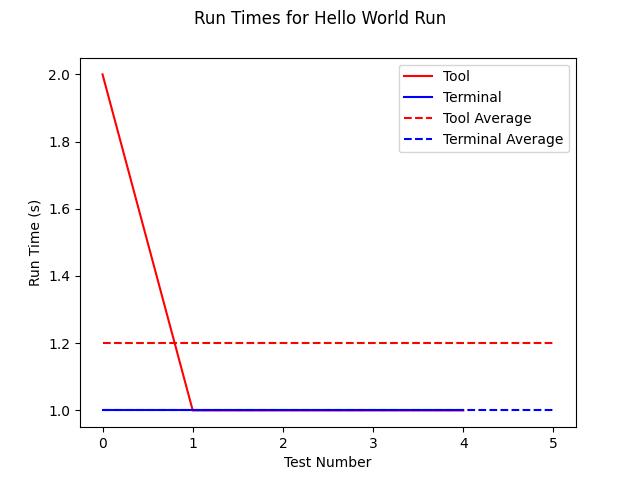
\includegraphics[width=3in]{images/evaluation/run5/hello-world}
  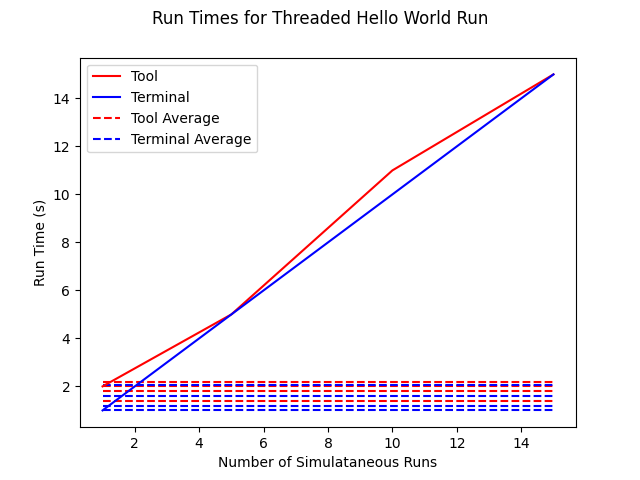
\includegraphics[width=3in]{images/evaluation/run5/thread-hello-world}
  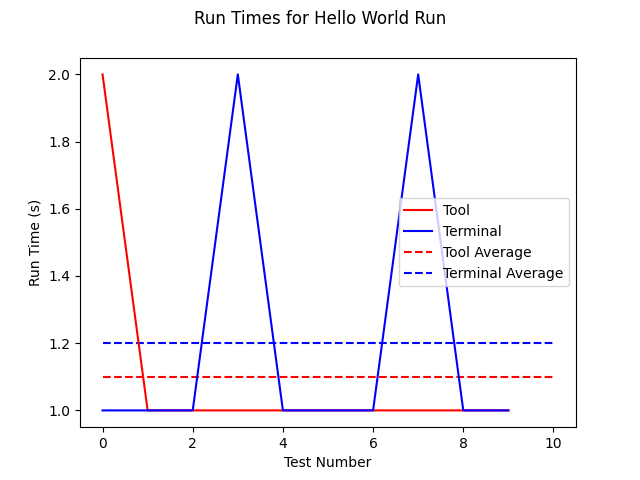
\includegraphics[width=3in]{images/evaluation/run6/hello-world}
  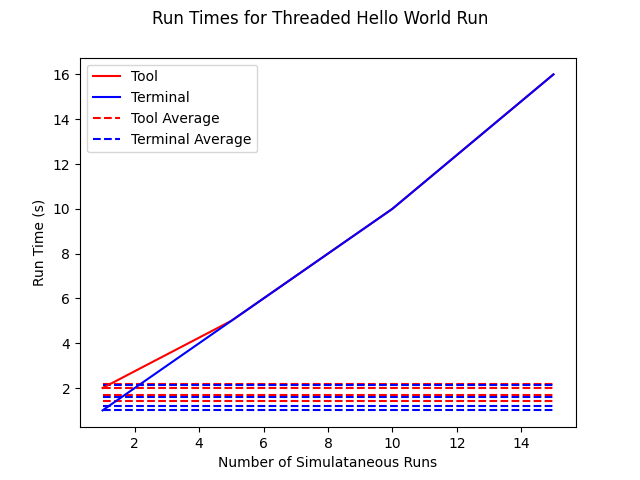
\includegraphics[width=3in]{images/evaluation/run6/thread-hello-world}
  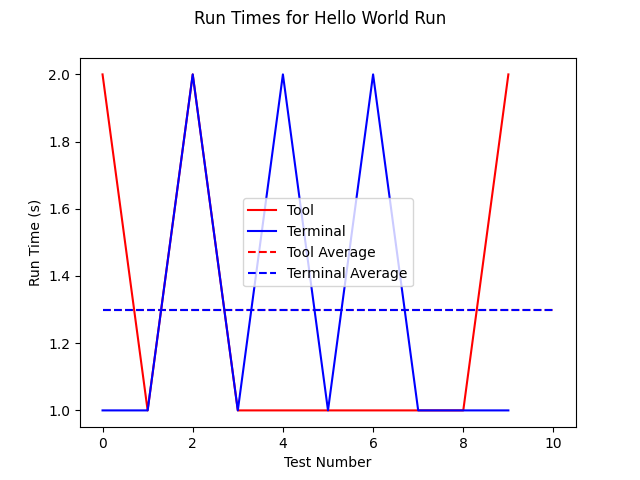
\includegraphics[width=3in]{images/evaluation/run7/hello-world}
  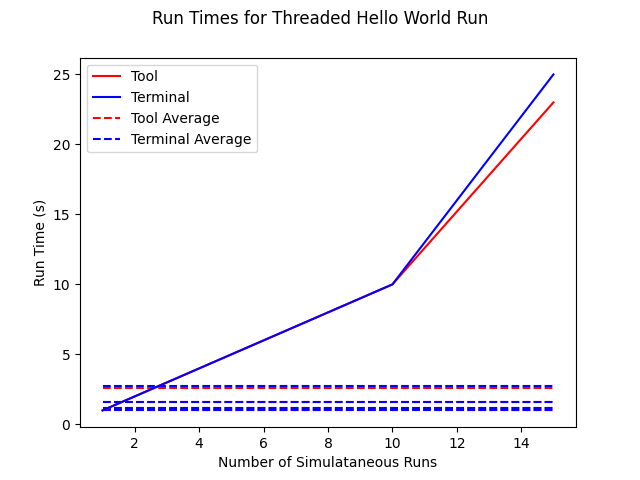
\includegraphics[width=3in]{images/evaluation/run7/thread-hello-world}
  \caption{Hello World Run Times}
  \label{img:helloWorld}
\end{figure}

\begin{figure}[h!]
  \centering
  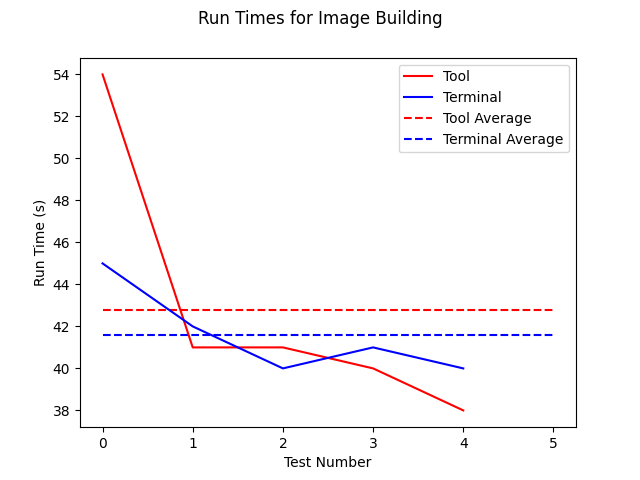
\includegraphics[width=3in]{images/evaluation/run5/image-build}
  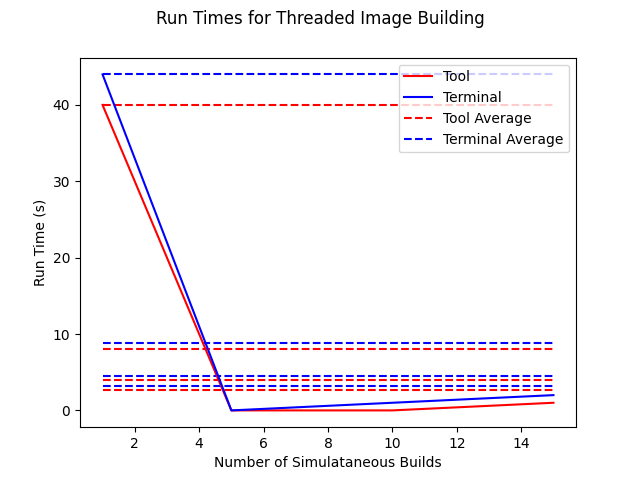
\includegraphics[width=3in]{images/evaluation/run5/thread-image-build}
  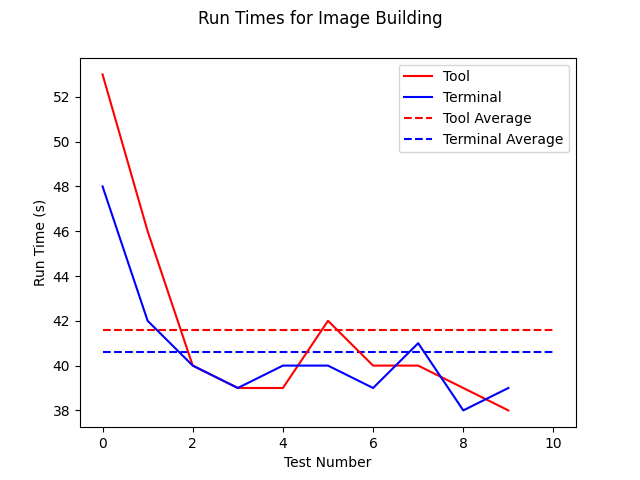
\includegraphics[width=3in]{images/evaluation/run6/image-build}
  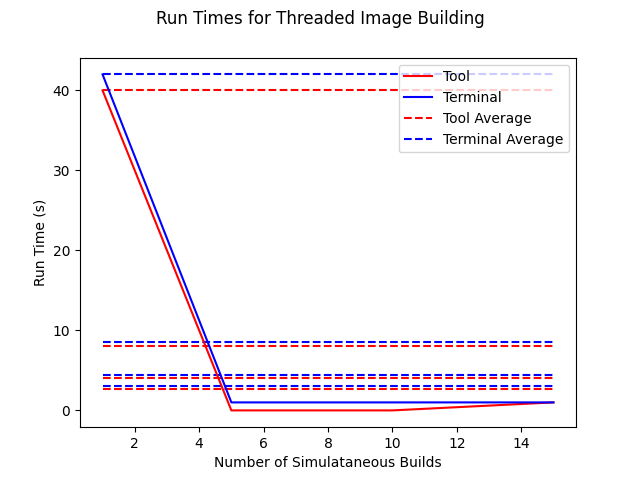
\includegraphics[width=3in]{images/evaluation/run6/thread-image-build}
  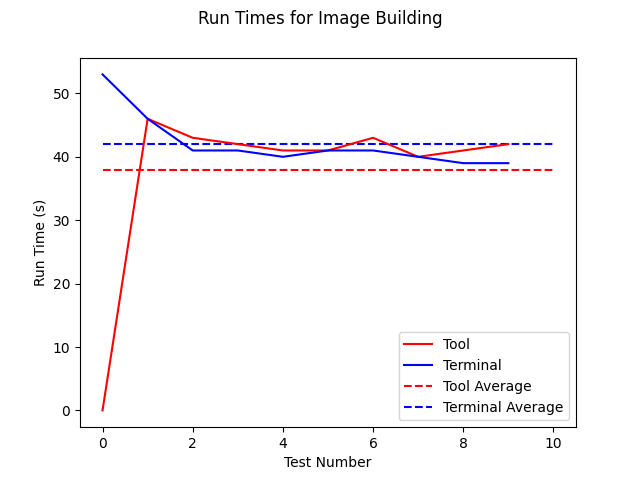
\includegraphics[width=3in]{images/evaluation/run7/image-build}
  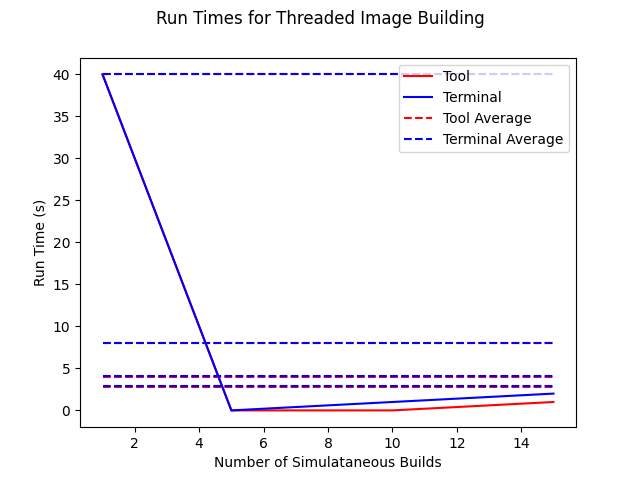
\includegraphics[width=3in]{images/evaluation/run7/thread-image-build}
  \caption{Image Build Run Times}
  \label{img:imageBuild}
\end{figure}

\begin{table}[h!]
\begin{tabular}{llllll}
Test Number & Test Type & \multicolumn{4}{l}{HELLO WORLD EVALUATION DATA}  \\
5           & Tool      & Times & 2, 1, 1, 1, 1                & Ave & 1.2 \\
            & Terminal  & Times & 1, 1, 1, 1, 1                & Ave & 1.0 \\
6           & Tool      & Times & 2, 1, 1, 1, 1, 1, 1, 1, 1, 1 & Ave & 1.1 \\
            & Terminal  & Times & 1, 1, 1, 2, 1, 1, 1, 2, 1, 1 & Ave & 1.2 \\
7           & Tool      & Times & 2, 1, 2, 1, 1, 1, 1, 1, 1, 2 & Ave & 1.3 \\
            & Terminal  & Times & 1, 1, 2, 1, 2, 1, 2, 1, 1, 1 & Ave & 1.3
\end{tabular}
\caption{Hello World Evaluation Data}
\label{tab:helloWorld}


\begin{tabular}{llllll}
Test Number  & Test Type  & \multicolumn{4}{l}{THREADED HELLO WORLD EVALUATION DATA}            \\
5            & Tool       & Times  & 2, 5, 11, 15  & Aves  & 2.0, 1.4, 1.8, 2.2                 \\
             & Terminal   & Times  & 1, 5, 10, 15  & Aves  & 1.0, 1.2, 1.6, 2.066666666666667   \\
6            & Tool       & Times  & 2, 5, 10, 16  & Aves  & 2.0, 1.4, 1.7, 2.2                 \\
             & Terminal   & Times  & 1, 5, 10, 16  & Aves  & 1.0, 1.2, 1.6, 2.1333333333333333  \\
7            & Tool       & Times  & 1, 5, 10, 23  & Aves  & 1.0, 1.2, 1.6, 2.6                 \\
             & Terminal   & Times  & 1, 5, 10, 25  & Aves  & 1.0, 1.2, 1.6, 2.7333333333333334  \\
\multicolumn{6}{l}{Note: Tests used the following number of threads for operations: 1, 5, 10, 15}
\end{tabular}
\caption{Threaded Hello World Evaluation Data}
\label{tab:threadHello}


\begin{tabular}{llllll}
Test Number & Test Type & \multicolumn{4}{l}{IMAGE BUILDING EVALUATION DATA}          \\
5           & Tool      & Times & 54, 41, 41, 40, 38                     & Ave & 42.8 \\
            & Terminal  & Times & 45, 42, 40, 41, 40                     & Ave & 41.6 \\
6           & Tool      & Times & 53, 46, 40, 39, 39, 42, 40, 40, 39, 38 & Ave & 41.6 \\
            & Terminal  & Times & 48, 42, 40, 39, 40, 40, 39, 41, 38, 39 & Ave & 40.6 \\
7           & Tool      & Times & 0, 46, 43, 42, 41, 41, 43, 40, 41, 42  & Ave & 37.9 \\
            & Terminal  & Times & 53, 46, 41, 41, 40, 41, 41, 40, 39, 39 & Ave & 42.1
\end{tabular}
\caption{Image Building Evaluation Data}
\label{tab:imageBuild}


\begin{tabular}{llllll}
Test Number  & Test Type  & \multicolumn{4}{l}{THREADED IMAGE BUILDING EVALUATION DATA}         \\
5            & Tool       & Times  & 40, 0, 0, 1  & Aves  & 40.0, 8.0, 4.0, 2.7333333333333334  \\
             & Terminal   & Times  & 44, 0, 1, 2  & Aves  & 44.0, 8.8, 4.5, 3.1333333333333333  \\
6            & Tool       & Times  & 40, 0, 0, 1  & Aves  & 40.0, 8.0, 4.0, 2.7333333333333334  \\
             & Terminal   & Times  & 42, 1, 1, 1  & Aves  & 42.0, 8.6, 4.4, 3.0                 \\
7            & Tool       & Times  & 40, 0, 0, 1  & Aves  & 40.0, 8.0, 4.0, 2.7333333333333334  \\
             & Terminal   & Times  & 40, 0, 1, 2  & Aves  & 40.0, 8.0, 4.1, 2.8666666666666667  \\
\multicolumn{6}{l}{Note: Tests used the following number of threads for operations: 1, 5, 10, 15}
\end{tabular}
\caption{Threaded Image Building Evaluation Data}
\label{tab:threadBuild}

\end{table}


\section{Threats to Validity}
\label{sec:threats}

There are several threats to the validity of both the tool, as well as the evaluation tests. The first threat comes from the evaluation itself, which is that there are many ways the data produced can be interpreted. This is an aspect that is inherent with any kind of evaluation and is present within this evaluation. However, I believe that the data, in this case, is rather straight forward to interpret.

The next possible threat to validity is the Threaded Image Building test, which as previously discussed, is a factor of how the tests were written and to fix would require other tests to be completely rewritten. However, despite these issues and admitting that they could pose a threat, I do not feel that they do. The tests show that it is possible with the tool to run multiple builds at the same time, however, there will never be a time for the same image to be built multiple times in parallel. So this test, while failing in one account, does succeed in illustrating the potential of the tool.

Looking directly at the tool several parts do not directly threaten its validity but do question how well the tool meets its goal. The first part that does this is the error handling, which is currently very basic and while it covers most issues does not handle some higher-level issues. The main case of this occurring is if the user (using the graphical interface) attempts to delete an image that doesn't exist, there is no indication that the image does not exist. These kinds of issues are being worked on and should be fixed by the time of the final release.

An additional threat that was discussed in a fair amount of detail back in section \ref{sec:eval} is the lack of evaluation of the Docker Installer. As previously discussed this is something I am hoping to figure out before the final version is due, but in the meantime, I do consider a threat to the validity of the tool. Not quite in the same vein as this is the threat posed by non-Linux operating systems, primarily Mac OS. This is an operating system that I do not have access to and as a result, will not be able to verify the compatibility of my tool. The installation commands which were loaded into the instruction set for Mac OS were taken directly from the Docker website, but with no way to ensure that they work with my tool, Mac OS exists as a threat to validity.

The final threat to the validity of my tool once again is on the evaluation suite itself. This is a suite that was written and designed by myself, which may mean there are areas of the tool which I should have evaluated that I have not. This could be for a variety of reasons, ranging from not believing it to be necessary to simply not knowing a feasible way to fully evaluate all of the work that has been done. This all being said, I believe that what I have evaluated are the core components of the tool which can be evaluated automatically and generate results that hold the lowest level of bias and the highest level of correctness as possible.

% How can the system break. How reliable is the tool?
